\documentclass[twocolumn, 9pt]{extarticle}
\usepackage[top=1in, bottom=1.25in, left=0.8in, right=0.8in]{geometry}
% \documentclass{article}
% \usepackage[top=1.5in, bottom=1.25in, left=1.8in, right=1.8in]{geometry}


%\usepackage{flushend} 
\usepackage[hyphens,spaces,obeyspaces]{url}
\usepackage{xurl}
\usepackage{multicol}
\usepackage{amssymb}
\usepackage{subcaption}
\usepackage{algorithm}
\usepackage{algpseudocode}
\usepackage{hyperref}
\hypersetup{colorlinks=true,linkcolor=black,citecolor=black, linktocpage}
% -- Single column version
%\documentclass[11pt]{article}
%\usepackage[top=1in, bottom=1in, left=1.5in, right=1.5in]{geometry}

\usepackage{lmodern}		% nice font
\usepackage[final]{microtype}	% better hyphenation

% Optional packages for enhanced functionality
\usepackage{graphicx} % For including images

\usepackage{tikz, lipsum}
\usetikzlibrary{positioning, decorations.pathreplacing, calc, arrows.meta, shapes.geometric}

\tikzset{
    bigbox/.style={draw, rounded corners, minimum width=2.0cm, minimum height=1.0cm},
    smallbox/.style={draw, rounded corners, minimum width=2cm, minimum height=1cm},
    bigcircle/.style={draw, circle, minimum size=2cm},
    bigellipse/.style={draw, ellipse, minimum width=3cm, minimum height=2.5cm},
    place/.style={inner sep=0pt, outer sep=0pt},
    fork/.style={decorate, decoration={show path construction, lineto code={
        \draw[rounded corners, ->](\tikzinputsegmentfirst)-|($(\tikzinputsegmentfirst)!.5!(\tikzinputsegmentlast)$)|-(\tikzinputsegmentlast);}
    }}
}

% \renewenvironment{abstract}
% {
%   \centerline
%   {\large \bfseries \scshape Abstract}
%   \begin{quote}
% }
% {
%   \end{quote}
% }
%

\title{Cardinality Estimation of Distinct Items - A Review}
\author{Sebastian Balsam}
\date{\today}

\newcommand{\todo}[1]{\textcolor{red}{#1}}

\begin{document}

\maketitle

\begin{abstract}
In this paper I want to give an overview of different solutions
for the Count Distinct Problem. I will follow the development from the
first algorithm by Flajolet and Martin, to the HyperLogLog algorithm 
and further optimizations to the Extended HyperLogLog algorithm, 
to increase the estimation quality while
at the same time decrease the memory consumption of these algorithms.
I have implemented most of the described algorithms to confirm the 
algorithms estimations and compare their results. This paper shows
the development of the algorithm over the last 40 years with the 
main changes and improvements.
\end{abstract}


\section{Introduction}

The cardinality estimation problem or count-distinct problem is about finding
the number of distinct elements in a data stream with repeated elements. These
elements could be URL's, unique users, sensor data or IP addresses passing
through a data stream. A simple solution would be to use a list and add an item
to this list each time we encounter an unseen item. With this approach we can
give an exact answer to the query, how many distinct elements have been
seen. Unfortunately if millions of distinct elements are present in a data
stream, with this approach, we will soon hit storage boundaries and the
performance will deteriorate. 

As we often do not need an exact answer, streaming algorithms have been
developed, that give an approximation that is mostly good enough and bound to a
fixed storage size. There different approaches to solve this problem. Sampling
techniques are used as an estimate by sampling a subset of items in the set and
use the subset as estimator, e.g. the CVM algorithm by Chakraborty et al.
\cite{cvm2023}. In its simplest form if we take a sample size of $N_0$ for a
set of size $N$, we get an estimate by counting the distinct items times
$N/N_0$. While sampling methods generally give a good estimate, they can fail
in certain situations. If rare elements are not in the sampled set, they would
not be counted and we would underestimate. Another problem is replicating
structures in the data. If we sample every 10th item, and accidentally every
10th item is different, while other items are mostly the same, we would
overestimate. For database optimization, machine learning techniques have been
used recently for cardinality estimation \cite{Liu2015, Woltmann2019,
Schwabe2024}. 

The technique I want to focus on in this paper are stochastic sketch techniques
that implement a certain data structure and an accompanying algorithm to store
information efficient for cardinality estimation. I will follow the development
chronologically from the first algorithm of Flajolet and Martin in 1985
\cite{fm85}, to the HyperLogLog algorithm in 2007 and the HyperLogLog++
algorighm in 2013 to the HLL-TailCut algorithm from 2017, the martingale
setting of HyperLogLog in 2017 and the ExtendedHyperLogLog in 2023. All of the
discussed methods are based on the original method by Flajolet and Martin and
we can follow the different problems and solutions researchers have found to
improve the algorithm further and further. From a science history perspective,
this paper presents in a chronological order all the improvements that have
been madeo, often with surprising ideas. There are other methods that solve the
given problem, as mentioned before, but I want to focus specifically on the
history of improvements of the Flajolet \& Martin algorithm.

I will omit any mathematical proofs, as they can be found in the original
sources, but I will specify any equations that are necessary for understanding
the algorithm. Most of the algorithms are implemented by myself in the
accompanying repository \cite{repo} and have been used to verify and confirm
the problems and results of the algorithms.
%\section{Probabilistic Counting with Stochastic Averaging}

%- Overview of PCSA
%- Problem description

\section{Flajolet and Martin}

Before the advent of the internet there were not many data stream applications
as we have today. But databases existed and began to grow in size. As table
sizes grew, evaluation strategies became important, how to handle such big data
tables for join operations. Query optimizers were developed that could find the
optimal strategy.

In this context Flajolet and Martin developed in 1985 a method to estimate the
number of distinct items in a set in a space efficient way\cite{fm85}. Often
this method is called Probabilistic Counting with Stochastic Averaging (PCSA)
in the literature, I will refer to it as FM85. The idea behind the method is to
use a hash function that maps $n$ items uniformly to integers. If we look at
the binary representation of these integers, and check the longest runs of
zeros, in about $n/2$ cases, we have a '0' at any position. In about $n/4$
cases, we have two '0's consecutively. With a chance of $1/8$ we have three '0'
in a row, and so on. That means if we start for example at the right and count
the zeros for each element in the stream, based on maximal number we have seen
so far, we can estimate the number of items. When we add an item, we use the
algorithm as described in Algorithm \ref{alg:fm85-add} to add set the position
of the rightmost '1' in a bitmap.

Flajolet and Martin found that they get better result, if an average of
multiple ($m$) registers of bitmaps are used. This is equivalent with running an
experiment multiple times to get results closer to the expected value. With a
higher number of registers available for the average, the estimation quality raises,
but at the same time more memory to store the bitmap is needed. They use the
hash value to decide the register  (by using the modulo operation) and save the
rightmost '1' of the binary representation in this register.

\begin{algorithm}
\caption{Adding an item in the Flajolet-Martin algorithm.}
	\label{alg:fm85-add}
	\begin{algorithmic}[1]
		\State $m \gets $ Number of registers
		\Function{$\phi$}{$val$}
			\State \Return position of the first 1 bit in val.
		\EndFunction

		\Function{addItem}{$x$}
			\State $hashedx \gets hash(x)$
			\State $\alpha \gets hashedx \textrm{ mod } m$
			\State $index \gets \phi(hashedx \textrm{ div } m)$
			\State $BITMAP[\alpha][index]=1$
		\EndFunction
\end{algorithmic}
\end{algorithm}

\begin{algorithm}
\caption{Get an estimate in the Flajolet-Martin algorithm.}
	\label{alg:fm85-query}
	\begin{algorithmic}[1]
		\State $m \gets $ Number of registers
		\Function{query}{}
			\State $\rho \gets 0.77351, S \gets 0$
			\State $\max \gets 32$ \Comment{32 bit per register}
			\For{$i:=0$ to $m-1$}
				\State $j \gets 0$
				\While{$BITMAP[i][j]==1$ and $j<max$}
					\State $j \gets j+1$
				\EndWhile
				\State $S \gets S+j$
			\EndFor
			\State \Return $int(m / \rho \cdot 2 ^{S/m})$
		\EndFunction
\end{algorithmic}
\end{algorithm}

When an estimate is needed, an average of the leftmost zeros over all registers 
are used, as shown in algorithm \ref{alg:fm85-query}. The magic number 
$\rho=0.77351$ is used, as the expected Value of R - the position of 
leftmost zero in the bitmap is 
$$
\mathbb{E}(R) \approx \log_{2}{\rho n}
$$
We sum up the registers and as each register only counted $1/m$ items,
we get an estimate with:
$$
E = \frac{1}{\rho} m \cdot 2^{\frac{S}{m}}.
$$

The results for this algorithm are shown in Figure 1. The memory consumption
for the algorithm is $m \cdot 32$. That means with $m=256$, we can produce estimates
with about 5\% standard error for higher cardinalities and have to use 
$256 \cdot 32=8192 \textrm{ bit } = 1 \textrm{kB}$ of memory to safely 
count up to 100 million items, before the quality decreases.

\begin{figure*}[htb]
	\begin{subfigure}{.33\textwidth}
		\centering
		\includegraphics[width=.9\linewidth]{fm85_16.pdf}
		\caption{m=16}
		\label{fig:fm85_16}
	\end{subfigure}%
	\begin{subfigure}{.33\textwidth}
		\centering
		\includegraphics[width=.9\linewidth]{fm85_64.pdf}
		\caption{m=64}
		\label{fig:fm85_64}
	\end{subfigure}
	\begin{subfigure}{.33\textwidth}
		\centering
		\includegraphics[width=.9\linewidth]{fm85_265.pdf}
		\caption{m=265}
		\label{fig:fm85_265}
	\end{subfigure}

	\caption{Results for the Flajolet Martin algorithm. The percentage of
	deviation from the true number of items over 30 runs (in gray) are shown
	(m=265) up to one million items. The red line shows the average over the 30
	runs.} 
	\label{fig:fm85} 
\end{figure*}

Figure \ref{fig:fm85} shows the results of my implementation of the FM
algorithm of a cardinality up to one million items for different values of $m$.
We can see that the algorithm results in strong overestimation below 1500 items
for $m=256$. After that, we only have a deviation on average of about 1 percent
of the true number of items. This makes sense, since we use 256 registers, each
new item is only stored in one of the registers, and many would remain empty in
the beginning. With $256/0.77=332$ and $s^{n/265}=1$ for low $n$ we
overestimate in the beginning. The solution for numbers below 1500 items is
simply to count these items exactly in an array, and only use Flajolet \&
Martin above a certain number.

The value of $m$ - the number of registers is important for accuracy. Even
though we have more overestimation for less items counted, we get a better
estimation for a higher number of items. With $m=265$, Flajolet and Marin
report a bias of 0.0073 and a standard error of 4.65\%. For $m=16$, we have a
bias of 1.0104, about the same, but a standard error of 19.63\%. These numbers
match my own experiments. Generally, as estimated later in \cite{Durand2003},
the standard error is about $1.3 / \sqrt{m}$.  

\section{HyperLogLog}

A first refinement of the Flajolet \& Martin algorithm came in 2003 by Durand
and Flajolet \cite{Durand2003}. Already in this paper the memory usage and the
standard error could be reduced. They introduced a truncation rule to only use
70\% of the smallest values in the registers, since they found that the arithmetic
mean would often overestimate. Later, in 2007 Flajolet \cite{Flajolet2007}
refined the algorithm even more to improve the accuracy even further to an
algorithm called HyperLogLog (HLL).

When we try to estimate the number of items, in the
FM85 algorithm, we look for the maximum number of '1' in the bit registers. All the other '1'
before and any bits after this position are not used. So instead of saving the
complete register, it should be enough to just save the maximum number. 
In addition, since we have a maximum of 32 bits originally in the
register, we only need 5 bits ($2^5=32$) for this number to be stored for each
register. This is an additional memory reduction. Instead of 1kB of memory as in the
original FM85 algorithm, the HLL algorithm only need 160 bytes.

\begin{algorithm}
\caption{Adding an item in the HyperLogLog algorithm.}
	\label{alg:hll-add}
	\begin{algorithmic}[1]
		\State $m \gets $ Number of registers
		\Function{$\phi$}{$val$}
			\State \Return position of the first 1 bit in val.
		\EndFunction

		\Function{addItem}{$x$}
			\State $hashedx \gets hash(x)$
			\State $j \gets hashedx \textrm{ mod } m$
			\State $w \gets \phi(hashedx \textrm{ div } m)$
			\State $M[j]:= max(M[j], \phi(w))$
		\EndFunction
\end{algorithmic}
\end{algorithm}

Algorithm \ref{alg:hll-add} shows my implementation of the algorithm to add an
item. The original version used
the first $b$ bits with $m=2^b$ to identify the register and used the remaining
bits to evaluate the maximum numbers of zeros. As my implementation is done in
python and integer values don't have a fixed size, I used the modulo operation
(the last $b$ bits) to identify the register index and div $m$ (the equivalent
of a bit shift $2^m$) as the remaining value to get the position of the first
1-bit. This should not change the outcome, and as our results are comparable
with the results of the HyperLogLog paper, this should not be a problem. 

As the original algorithm would overestimate when calculating the average over
all registers. Only using the lowest 70\% was one method to improve the
results. For HLL, Flajolet used the harmonic mean given by 
$$ 
H = \frac{n}{\sum_{j=i}^n \frac{1}{x_i}} 
$$ 
instead of the arithmetic mean to get
the average of the registers against overestimation, as the harmonic mean gives
lower results. The raw estimate (before corrections) is calculated with 
\begin{equation} \label{eq1}
E = \alpha_m m^2 \cdot \left(\sum_{i=1}^m 2^{-M[i]} \right)^{-1} 
\end{equation}
Since each register will have $n/m$ elements, when $n$ is the number of
counted elements so far, with the harmonic mean of these
registers $mH$ would be about $n/m$. Therefore, $m^2H$ should be $n$. Again
a constant $\alpha$ is used to correct the bias due to hash collisions.

In addition, Flajolet introduced corrections for very low numbers where we would
not have enough data for good predictions and would see overestimations as in
the original FM algorithm as shown in Figure \ref{fig:hll-flow}. If the estimate $E$ is below $\frac{5}{2}m$,
they use linear counting and get a correction of
\begin{equation} \label{eq2}
E^* = m \log(\frac{m}{V})
\end{equation}
with $V$ being the number of registers equal to $0$. Instead of using the number of
bits calculated by the harmonic mean over the registers, we estimate by counting
the number of empty registers. As most of the registers are empty anyway this gives
a result, much closer to the true value of the number of items
For very high numbers, where hash collisions are more common, they give another
correction, based on the probability of hash collisions.

\begin{figure}
\centering
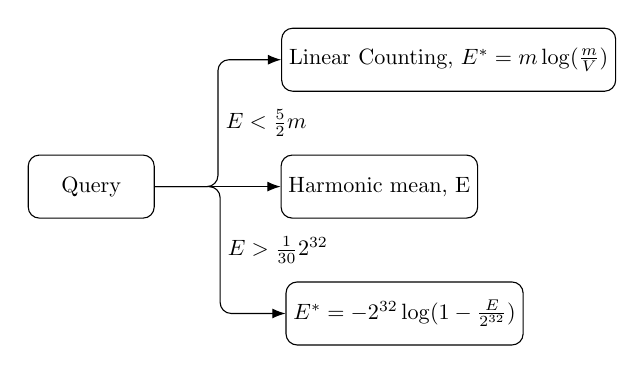
\begin{tikzpicture}[scale=.8, transform shape, node distance=1cm, >=Latex]
	\node(Query)[bigbox]{Query};
	\node(Harmonic)[bigbox, right=of Query, xshift=1.0cm]{Harmonic mean, E};
	\node(Below)[bigbox, above=of Harmonic, xshift=1.1cm]{Linear Counting, $E^*=m\log(\frac{m}{V})$};
	\node(Above)[bigbox, below=of Harmonic, xshift=0.4cm]{$E^*=-2^{32}\log(1-\frac{E}{2^{32}})$};
	\draw[->](Query.east)--(Harmonic.west);
	\draw[fork](Query.east)-- node[anchor=west] {$E < \frac{5}{2}m$} (Below.west);
	\draw[fork](Query.east)-- node[anchor=west] {$E > \frac{1}{30}2^{32}$}(Above.west);
\end{tikzpicture}
	\caption{When an estimation for HLL is queried, corrections are made for
	very small and very large cardinalities, while most of the estimates are
	generated by the harmonic mean calculation.}
	\label{fig:hll-flow}
\end{figure}

Figure \ref{fig:hll256} shows the results for one million items, and we
can see, that the results are good, even for few items. 

\begin{figure}[htb]
	\includegraphics[width=1.0\linewidth]{hll_256.pdf}
	\caption{The results of the error in percentage of one
	million items for the HyperLogLog algorithm over 30 independent runs
	for $m=256$. By using linear counting for lower cardinalities, the problem
	of FM85 in this area is solved.}
	\label{fig:hll256}
\end{figure}

Overall the quality of HLL exceeds the FM algorithm both in space and
estimation quality and has become the standard in many applications
\cite{redis2025, dragonfly2025, redshift2025}. It is memory efficient, is fast, as the
slowest part is the hashing function, scalable up to $10^9$ without loss of
quality, simple to implement and has a standard error of only $1.04/\sqrt{m}$.

Originally developed for use in databases, both FM85 and HLL have become more
interesting for streaming applications too. \cite{Scheuermann2007} propose a
lossless compression scheme with arithmetic coding that produces results close
to the theoretical optimum to perform distributed data aggregations over networks.

\section{HyperLogLog++}

The next improvement came in 2013 by \cite{Heule2013} with HyperLogLog++
(HLL++). In their paper they use a 64-bit hash function, that reduces hash
collisions for lower cardinalities. Instead of using 5 bits to store the
maximum '1's in registers, they use 6 bits. With this change they are able to
securely estimate cardinalities up to $2^{64} = 1.8\cdot 10^{19}$. Even though
this is a number that seldom should be met in real life, they propose to add an
extra bit even more, if needed, as memory is cheap compared to the amount of
items at this cardinality.

With this higher number of storage, since hash collisions are not a problem
anymore, the correction for large cardinalities used in HLL, is also not needed
anymore. For small cardinalities below $\frac{5}{2}m$, they keep the linear
counting correction of HLL as in equation (\ref{eq2}). 

% \begin{figure}[htb]
% 	\includegraphics[width=1.0\linewidth]{hll_16380.pdf}
% 	\caption{Spike at the transition between linear counting and harmonic mean
% 	estimation in HLL for $m=16384 = 2^{14}$.}
% 	\label{fig:hll_spike}
% \end{figure}
\begin{figure*}[thb]
	\begin{subfigure}{.5\textwidth}
		\centering
		\includegraphics[width=0.9\linewidth]{hll_16380.pdf}
		\caption{HLL with spike at transition.}
		\label{fig:hllspike}
	\end{subfigure}%
	\begin{subfigure}{.5\textwidth}
		\centering
		\includegraphics[width=.9\linewidth]{llbeta_16380.pdf}
		\caption{LogLogBeta without a spike.}
		\label{fig:llbetaspike}
	\end{subfigure}
	\caption{Figure (a) shows a spike at the transition between linear counting and harmonic mean
	estimation in HLL for $m=16384 = 2^{14}$ at $\frac{2}{5}2^{14}$. 
	With the HLL++ and LogLogBeta algorithm,
	this spike is eliminated as shown in figure (b).}
	\label{fig:hll_spike} 
\end{figure*}

Another improvement of HLL++ is the use of Bias correction. They show that the
transition between linear counting of small values and harmonic mean estimation
of higher values is not flawless. Figure \ref{fig:hllspike} shows a spike at
the transition. This spike is not visible for all values of $m$, but for some,
it might be a problem. Instead, they used 200 cardinalities as interpolation
points get an estimate for bias correction values by using k-nearest neighbor
interpolation. This not only reduced the spikes at the transition points
between linear counting and the harmonic mean estimation, but gives better
general results also for higher cardinalities. I have to point out, that
only the bias will be corrected, the standard error for HLL++ and HLL is
about the same (except for the spike reduction).

Since 5 bits are used to store the data, Heule et al. saves the number of '1's
with a sparse representation as long as the size of the sparse representation
is smaller than $6 \cdot m$ bits. In this way, they can keep the size
requirements still small, in fact, as long as $n < m$, HLL++ requires
significantly less memory than HLL. For higher cardinalities this is of course
not true anymore, since we can not use sparse representations.

To summarize HLL++, they use 6-bit instead of 5 bits, but a sparse
representation for small cardinalities to save memory. The process of counting
a new item is otherwise unchanged and done, as proposed in the HLL algorithm.
Using 6-bits leads to better estimations of higher cardinalities, so a
correction for high cardinalities is not needed anymore. With empirical bias
corrections they improve the estimation by adjusting the bias and prevent
spikes.

\section{LogLogBeta}

In 2016, \cite{Qin2016} used the results of HLL++ to improve the algorithm
even further. While HLL++ still needed linear counting for small cardinalities
and a bias correction to handle the transition between linear counting and
the usual harmonic mean calculation, LogLog-$\beta$ (LogLogBeta) simplifies
this process to one function for the query operation. Otherwise, LogLogBeta
also uses 6 bits and a sparse representation as HLL++ does.

The modified version LogLogBeta proposes uses a function of $m$ and $z$ (the
number of empty registers), that also uses precalculated coefficients for
different values of $m$, that had been found empirically to correct the bias.
The update of the registers, when new items are counted is still done in
the same way as proposed for HLL and HLL++, but the query for the number
of items is now simplified to:

$$
E = \frac{\alpha_m M(m-z)}{\beta(m,z)+ \sum_{i=0}^{m-1}2^{-M[i]}}
$$

With $z=0$, $\beta(m,0)=0$ and this formula is the same as Flajolet used in 
the HLL algorithm equation (\ref{eq1}), so the changes apply only for situation where some of the
registers are 0. This is therefore a simplification and correction for
small cardinalities. The calculation for a given cardinality $c$ for $\beta(m,z)$
is given as an approximation of
$$
\beta(m,z) = \frac{\alpha_m m(m-z)}{c}-\sum_{i=0}^{m-1}2^{-M[i]}
$$
by calculating
$$
\beta(m,z) = \beta_0(m)z + \beta_1(m)z_l + \ldots + \beta_k(m)z_l^k
$$
with $z_l=\log(z+1)$. Here $\beta_k$ can be precalculated for different
values for $m$, which makes this calculation very efficient.

As we can see in Figure \ref{fig:llbetaspike}, the spike at the transition
between linear counting and the harmonic mean estimation is no longer visible.
In comparison to HLL++ the LogLogBeta algorithm might not be an improvement of
estimation quality, but is a great simplification of the algorithm and also
solves the problem of the transition between linear counting and harmonic mean
estimation.

\section{HLL-TailCut}
%https://topoer-seu.github.io/PersonalPage/csqjxiao\_files/papers/INFOCOM17.pdf
Already in \cite{Durand2003}, Flajolet only used the lowest 70\% of the registers.
This idea has been taken up by \cite{Xuao2017}. If we take a look at the histogram
of the numbers of values in the saved registers as shown in Figure \ref{fig:histogram},
we can see that the histogram has a long tail to the right, with few registers of
high values. These registers are not contributing very much to the result in the
calculation of the mean. But at the same time, they take precious memory. The 
general idea is to cut registers with higher values, which can save memory.
If we only store registers up to a size of 16, we only need 4 bits.

% \begin{figure}[htb]
% 	\includegraphics[width=1.0\linewidth]{llbeta_histogram.pdf}
% 	\caption{This histogram shows the frequency of the numbers in the registers for
% 	LLBeta with $m=2^{16}$ for 10 Million items. Even though, they are not visible in the figure, there
% 	are values up to 28, although with a very low frequency. That means we have a long
% 	tail to the right side with registers of little information.}
% 	\label{fig:histogram}
% \end{figure}
\begin{figure}[thb]
	\begin{subfigure}{.25\textwidth}
		\centering
		\includegraphics[width=0.9\linewidth]{llbeta_histogram.pdf}
		\caption{Histogram}
		\label{fig:hllspike}
	\end{subfigure}%
	\begin{subfigure}{.25\textwidth}
		\centering
		\includegraphics[width=.9\linewidth]{llbeta_histogram_log.pdf}
		\caption{Histogram with log scale}
		\label{fig:llbetaspike}
	\end{subfigure}
	\caption{This histogram shows the frequency of the numbers in the registers for
	LLBeta with $m=2^{16}$ for 10 Million items. Even though, they are not visible 
	in the left figure, there are values up to 28, although with a very low 
	frequency, as shown in the log scaled histogram on the right. That means we have a long
	tail to the right side with registers of little information as shown on the right with 
	the log scale.}
	\label{fig:hll_spike} 
\end{figure}

Registers with a maximum value of 16, can count up to $2^{16}=65536$. But since
we distribute the counted items on $m$ registers, we have $m\cdot 2^{16}$. As
$m$ is bound to a given estimation error, and we would like to minimize this error,
values for $m=2^{14}$ are quite common to get an estimation error of about 0.4\%.
This means we can store up to $2^{14}\cdot 2^{16} = 10^{9}$ items, although we 
get wrong results already before due to hash collisions. Nevertheless, this should
be enough for most applications.

Xuao et al. went further and could truncate the size to even $3\cdot m$ bits
by using a base register $B$ below the truncated registers $M$, as most of the
registers would share the same base register with increasing items that are counted.
They claimed they could reduce the error to $1.0/\sqrt{m}$, but \cite{Pettie2020} showed,
that this is unfortunately not true, the error is constant and independent of $m$. 
But \cite{Apache2019} has an implementation which uses 4 bits. The method of
tail cutting works and can reduce the amount needed for memory with 20\% (from 5 bits
to 4 bits).

\section{Mergeble sketches and Martingale settings}

In 2007, Daniel Ting \cite{Ting2014} found another method for better predictions.
If the different items are presented as a stream, we can view this stream as a
Markov process with martingale properties, that means the expected value of the 
next observation is equal to the most recent value. We can now use the
sketch as a predictor with Markov probabilities. The changes in the algorithm
are minimal. Every time the sketch is updated, we calculate the probability with 
$$
	q(S) = \frac{1}{m}\sum_{i=1}^m 2^{-S[i]}
$$
and we can update the martingale Estimator $N$ with
$$
	N_{new} = N + \frac{1}{q(S)}.
$$

The idea behind this is, that the sketch in its consecutive updates forms
a Markov process and this series of updates contains information that would
be thrown away in a mergeable setting. But if we follow the series, we can
use it to derive an estimator from the process as a whole. This is the 
martingale estimator, that is updated in each step for a new unseen item.

\begin{figure}[htb]
	\includegraphics[width=1.0\linewidth]{martingale.pdf}
	\caption{Mean squared error of HLL and HLL in martingale setting for cardinalities up to $10^6$ and $m=2^8$ The average
	MSE for EHLL is 0.0056, the avg. MSE for HLL is 0.0086. }
	\label{fig:martingale}
\end{figure}

Figure \ref{fig:martingale} shows the result for my implementation of the HLL
sketch in martingale setting, and we can see that this estimation is much
better than the plan HLL sketch. The plain HLL sketch needs about 1.5 more bits
than the martingale version for the same estimation quality. But there is one
catch to this. Since each estimate depends on the prior result, the sketch can
not be run in parallel in multiple threads.
We do not need any additional memory for the martingale enhancement of the
sketch, as we only need to update the value of the estimator, each time we
update the sketch. There is only one additional float value to store.

All other sketches that have been presented so far are mergeable sketches, that
means we can count items in different threads or on different locations and 
can merge the result, simply by merging the registers and get a new  
estimation. In a martingale setting, this is no longer possible. But for most
streaming applications, that would not be a problem, as long as the algorithm
can follow the entire stream and we don't process different sources on multiple 
locations. The martingale setting is therefore a big improvement for this algorithm. 

\section{Using Additional Bits}
%https://arxiv.org/pdf/2106.06525

Another new development came in 2021 when Tal Ohayon\cite{Ohayon2021} published
ExtendedHyperLogLoc (ExHLL). His method can be seen as a compromise between
FM85 and HLL. Ohayon saves the highest '1' exactly as in HLL. But in addition,
we also save in an additional bit for each register if the update with the highest
'1' was more than a single increment. In the FM85 algorithm, we counted the 
number of consecutive highest values. That means a FM85 register of '111000'
had the same result as '1110010'. Here the first three '1' would be used for estimation.
But HLL used the highest '1' in the register. In our example, the values for estimation
would be different for both registers - 3 and 6. 
ExHLL uses both, the maximum '1', and the information if the bit below the maximum '1'
would also be a '1' or a '0'. This gives additional information that can improve
the estimation quality.

Of course, since we have to use an additional bit per register, we have to use 6 bits
instead 5 bits, that were used for HLL. Algorithm \ref{alg:ehll-add} shows the 
algorithm if we want to add an item to the sketch. Here we have an array $C_1$ of size $m$
as we had in HLL, but in addition we keep track of the bit before the leading zero with 
the bitmap $C_2$.

\begin{algorithm}
\caption{Adding an item in the Extended HyperLogLog algorithm.}
	\label{alg:ehll-add}
	\begin{algorithmic}[1]
		\State $m \gets $ Number of registers
		\State $C_1$ array of size $m=2^b$ initialized with zeros
		\State $C_2$ bitmap array of size $m=2^b$ initialized with  ones
		\State $\phi(val)$ returns the position of the first 1 bit in val

		\Function{addItem}{$x$}
			\State $hashedx \gets hash(x)$
			\State $j \gets hashedx \textrm{ mod } m$
			\State $y \gets \phi(hashedx \textrm{ div } m)$
			\If{$\phi(y) = C_1[j] + 1$}
				\State $C_1[j] \gets \phi(y)$
				\State $C_2[j] \gets 1$
			\ElsIf{$\phi(y) > C_1[j] + 1$}
				\State $C_1[j] \gets \phi(y)$
				\State $C_2[j] \gets 0$
			\ElsIf{$\phi(y) = C_1[j]-1 $ and $C_2[j] = 0$}
				\State $C_2[j] \gets 1$
			\EndIf
		\EndFunction
\end{algorithmic}
\end{algorithm}

When the sketch is queried, we use the formula:

$$
E = \gamma m^2 \cdot \left( \sum_{j=1}^m 2^{-C_1[j]} + (1 - C_2[j]) 2^{-C_1[j]+1}) \right)^{-1}
$$

The first part is the same as equation (\ref{eq1}), that was used in HLL. But now
we use the additional $(1-C_2[j]) 2^{-C_1[j]+1}$. If $C_2[j]=1$, we get the
same calculation as in HLL, as the second term becomes 0. But if $C_2[j]=0$, we
add the probability $2^{-C_1[j]+1}$ that $C_1[j]-1$ would be used to generate
the predicted value. Since we use probabilities for $C_[j]$ and possibly
$C_1[j]-1$, the correction $\alpha$ we used for HLL is no longer valid and the
authors analyze the Expectation and variance to get the correction constant
$\gamma_m$.

This algorithm is an improvement to the standard HLL, but even though
the quality is much better, we have to be aware of the fact, that we 
still need linear counting for lower cardinalities and a correction for
very large cardinalities as Flajolet used in HLL. We also still see here
the spike at the transition between linear counting and the LogLog counting,
that can be corrected with the methods described in HLL++ and HLLBeta.

\begin{figure}[htb]
	\includegraphics[width=1.0\linewidth]{mse.pdf}
	\caption{Mean squared error of HLL and EHLL for cardinalities up to $10^6$ and $m=2^8$ The average
	MSE for EHLL is 0.0037, the avg. MSE for HLL is 0.0046. }
	\label{fig:mse}
\end{figure}

Figure \ref{fig:mse} shows the MSE of EHLL and HLL with values for $m$ chosen in a way, 
that both methods would use the same memory ($m_{EHLL} = 6/5 m_{HLL}$). The figure
shows that we get a lower error for EHLL than for HLL with the same memory
usage. The difference of these results are valid even in a martingale setting
as Ohayon can show.
%(https://arxiv.org/pdf/2308.16862)


\begin{figure}[htb]
	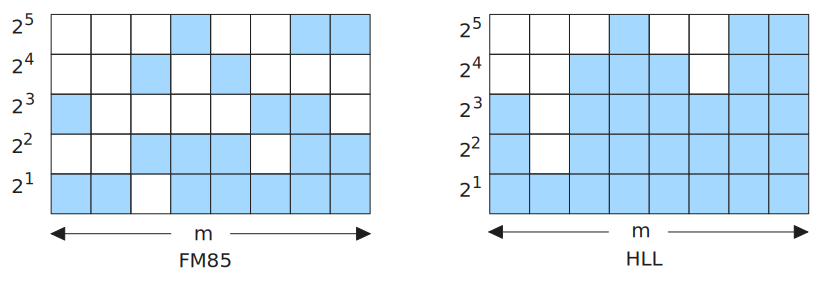
\includegraphics[width=1.0\linewidth]{hll.pdf}
	\caption{The left side shows the registers vertically that are used to 
	store the sketch for FM85. FM85 only uses the lowest consecutive marked areas.
	The right side shows the same situation for HLL.
	As it only stores the maximum values, any information on lower bits are lost. }
	\label{fig:hll-fm85}
\end{figure}

\cite{Wang2023} expanding an idea of \cite{Ting2014} of viewing the sketch as a
dartboard, where we would count the number of free cells of the bitmap sketch
(Generalized Remaining Area - $GRA$). While FM85 stored the complete bitmap, it
only used the lower marked bits and would give an estimate based on the number
of consecutive lower bits as shown in Figure \ref{fig:hll-fm85}. HLL only used
the maximum value for estimation to save some memory, but useful information is
lost in this sketch, as we would ignore some of the empty spaces in the bitmap.
Using less memory meant, we could use more registers for higher accuracy. But
using additional bits below the maximum bit would be useful, even though it
would also mean to need extra memory. The problem is, to find the optimal
tradeoff.

Otmar Ertl builds upon this idea in \cite{Ertl2024, Ertl2025}. In HLL we only
updated the maximal rightmost '1' in the sketch. EHLL saves in addition the bit
left of the rightmost '1' ($d=1$), one bit below the maximum value. Ertl
generalized this idea further. If we save the 2 bits left of the rightmost '1',
we have $d=2$. The original FM85 algorithm, that saved all bits used $d =
\infty$ even though this would be the theoretical limit as only 32 bits were
saved as a maximum. Ertl compares the memory usage of $d$ with the variance of
the error to find the optimal values for the memory-variance-product (MVP).
$d=2$ can be proven to be optimal to get the best ratio between memory efficiency and
low variance. The algorithm of UltraLogLog and ExaLogLog also specifies
corrections for small and large ranges of cardinality and analyzes performance
and compression possibilities.


\section{Conclusion}

\begin{table*}[t]
\label{tbl:methods}
\caption{Table showing a list of the presented methods with their estimation
	quality.}
\begin{center}
\begin{tabular}{ l l l l l }
	Algorithm & Year & Error & Memory & Comment \\ 
\hline
	FM85 & 1985 & $1.3/\sqrt{m}$ & $32\cdot m$ & probabilistic counting of bits \\
	HLL & 2007 & $1.04/\sqrt{m}$ & $5\cdot m$  & harmonic mean, corrections for small and big cardinalities \\
	HLL++ & 2013 & $1.04/\sqrt{m}$ & $\leq 6\cdot m$ & using 6 bits, empirical bias correction \\ 
	HLL Martingale & 2014 & $<1.04/\sqrt{m}$ & $5 \cdot m$ & non mergeable sketches \\ 
	LogLogBeta & 2016 & $1.04/\sqrt{m}$ & $\leq 6\cdot m$ & better quality for low cardinalities\\
	HLL-TailCut & 2017 & $1.04/\sqrt{m}$ & $4 \cdot m$ & truncated registers for lower memory consumption\\ 
	ExHLL & 2023 & $<1.04/\sqrt{m}$ & $6 \cdot m$ & using 1 additional bit below maximum per register\\ 
\end{tabular}
\end{center}
\end{table*}

In this paper I wanted to show the progressive improvements, that were made on
an algorithm, that already was based on an impressive idea 40 years ago. Each
update was made because of a certain need to solve a problem or to improve the
quality even further.

The original FM85 algorithm had problems for lower cardinalities and general
estimation error. Flajolet himself improved this with the HLL algorithm. By
only storing the maximum values per register, the sketch would need less space.
This means with the same space requirements, we can use more registers and thus
gain better quality. He also improved the prediction quality for lower
cardinalities by using linear counting, where we would not have enough
information in the lower registers. But the transition between linear counting
and the harmonic mean was not flawless. For certain values of $m$, we could see
a spike with overestimation. HLL++ and HLLBeta improved the estimation and
could eliminate the spike at the transition. HLL used 5 bits to save the values
for each register, but in the HLL-TailCut algorithm, it could be shown, that
already 4 bits can be enough to store big cardinalities without loosing quality
of estimation. Only a few registers have very high numbers that would not
contribute much to the estimation. They can be ignored, which means, we need
fewer bits to store the maximum values. Then again, using extra bits below the
maximum value for each register can be used to improve the quality even
further. EHLL uses one extra bit, and UltraLogLog even two extra bits for the
lowest memory-variance-product, as it can be proven that there is an optimal
balance between memory and estimation quality. We also saw, that if we do not
need the sketch to be mergeable, we can use a martingale estimator of the
sketch, that would improve the estimation quality even more.

There are some threats for validity that have to be mentioned here for this
paper. This is a narrative and not a systematic review. My choice for inclusion
of journal articles is based on a subjective views, which algorithms and
methods are important. My weighting for importance is mostly based on citations
in later journal articles and search results in Google Scholar and Semantic
Scholar. 

Implementations to verify a method or to visualize a problem, mostly to
generate the included figures can contain errors, even though they confirm the
original results. Most of my implementations contain simplifications to
visualize a certain aspect of a problem, while ignoring other points. My
implementations are done in Python and I focused mostly on the error of
estimation. The memory saving aspect of most methods is not implemented in my
solutions (registers on a bit level), as I did not focus on it. In a lower
level language this could be implemented very easy, but would not change the
results of the included figures.

We can see, that the development of Flajolet's original sketch has not stopped
in the last 40 years and researchers still find better ways to improve on the
idea by adding new insights and building upon their predecessors. 


\small
\bibliographystyle{apalike}
\bibliography{bibfile}

\end{document}
